\documentclass[aspectratio=169,11pt,hyperref={colorlinks=true}]{beamer}
\usepackage[utf8]{inputenc}
\usepackage[T1]{fontenc}
\usepackage{fontspec}
\usepackage[absolute,overlay]{textpos}
\usepackage{listingsutf8}
\usepackage{listings-golang}
\usepackage{tikz}
\usepackage{color}
\usepackage{fontawesome5}
\usepackage{svg}


\title{Adopting CDEvents and Embracing Interoperability}
\date[9 May 2023]{cdCon + GitOpsCon | 9 May 2023 | \faTwitter ~@\_cdevents | \faGithub ~cdevents}
\author[Andrea Frittoli]{%
  Andrea Frittoli \\
  Developer Advocate @ IBM\\
  andrea.frittoli@uk.ibm.com \\
  \faTwitter ~@blackchip76 | \faGithub ~afrittoli\\
  ~\\
  Session: \href{https://sched.co/1KUH8}{sched.co/1KUH8}
}

\usetheme{af}

% Code style
\setlststyle

\lstdefinelanguage{koyaml}{
  keywords={github, com, afrittoli, examples, ms, go, helloworld},
  sensitive=false,
  comment=[l]{\#},
  morestring=[b]',
  morestring=[b]"
}

% Automatic section frame
% \AtBeginSection{\frame{\sectionpage}}

\begin{document}

\begin{frame}
\titlepage{}
\end{frame}

\begin{speakerframe}[af_wind.jpg]{Andrea Frittoli}%
  {%
  \faGithub ~afrittoli | \faLinkedin ~andreafrittoli | \faTwitter ~@blackchip76
  }%
  {%
  \begin{itemize}
    \item{Open Source Advocate @ IBM}
    \item{Lives in Wales, enjoys the wind}
    \item{CDEvents maintainer, Events SIG co-chair}
    \item{Chair of CDF Technical Oversight Committee \\ Governing Board}
  \end{itemize}
  }%
\end{speakerframe}

\begin{lpicrblack}[calum-lewis-vA1L1jRTM70-unsplash.jpg]{%
  Photo by \href{https://unsplash.com/@calumlewis}{\underline{Calum Lewis}}, CC0
  }%
  {%
  \tableofcontents
  }%
  {}
  \frametitle{~~~~~~~~~~~~~~~~~~~~~~~~~~~~~~~~~~~~~~~~~~~~~~~~~~~Contents}
\end{lpicrblack}

\section[CDEvents]{A common specification for Continuous Delivery events}

\begin{grayframe}
  \frametitle{Continuous Delivery Pipeline}
  \begin{textblock*}{0.70\paperwidth}(0.15\paperwidth,0.20\paperheight)
    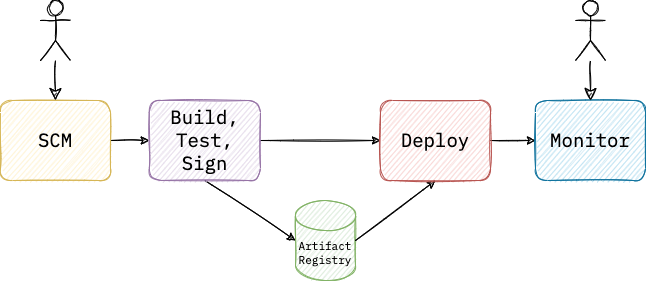
\includegraphics[width=0.70\paperwidth]{img/cdevents-1-no-events.png}
  \end{textblock*}
\end{grayframe}

\begin{grayframe}
  \frametitle{Integrations}
  \begin{textblock*}{0.70\paperwidth}(0.15\paperwidth,0.1\paperheight)
    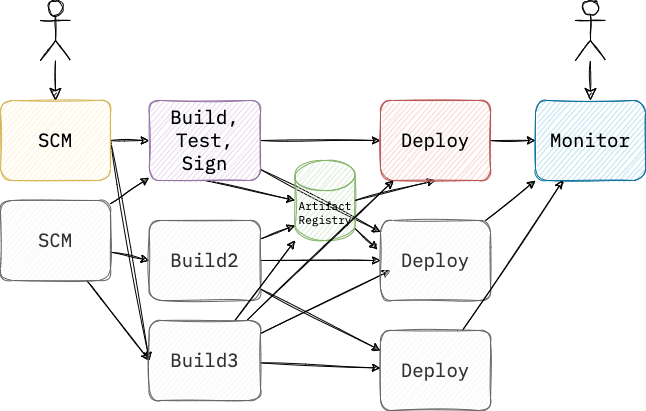
\includegraphics[width=0.70\paperwidth]{img/cdevents-2-no-events-multiple.png}
  \end{textblock*}
\end{grayframe}

\begin{whitetextontwopics}[shutterstock_1044739930.jpg]{%
  % by Igor Bulgarin
  % Shutterstock editorial license: https://support.shutterstock.com/s/article/Premier-Editorial-Content?language=en_US
  % https://www.shutterstock.com/image-photo/dnipro-ukraine-march-12-2018-four-1044739930
  Orchestration
  }{shutterstock_1483333925.jpg}{%
  Choreography
  % by A_Lesik
  % Shutterstock editorial license: https://support.shutterstock.com/s/article/Premier-Editorial-Content?language=en_US
  % https://www.shutterstock.com/image-photo/odessa-ukraine-july22-2019-ballet-classical-1483333925
  }%
  \frametitle{Orchestration vs. Choreography}
\end{whitetextontwopics}

\begin{sectionwithpicmediumcentral}[cdeventscon-gradient-16-9.jpg]{}
\end{sectionwithpicmediumcentral}
\note[itemize]{
  \item How many of you are familiar with CDEvents?
  \item Let's take a step back
  \item Why events in Continuous Delivery?
}

\begin{grayframe}
  \frametitle{Interoperability}
  \begin{textblock*}{0.70\paperwidth}(0.15\paperwidth,0.1\paperheight)
    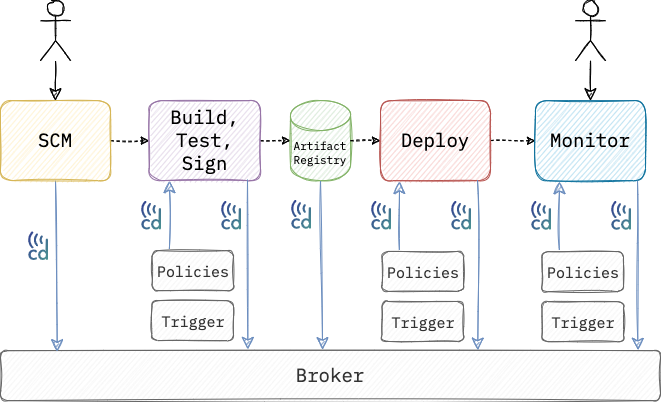
\includegraphics[width=0.70\paperwidth]{img/cdevents-3-events.png}
  \end{textblock*}
\end{grayframe}
\note[itemize]{
  \item Event driven workflows
  \begin{itemize}
    \item Scalable
    \item Decoupled
    \item Flexible
    \item Policy Driven
  \end{itemize}
  \begin{itemize}
    \item Multiple sources to trigger build
    \item Multiple sources to trigger Deployment
    \item Multiple listeners to build events
    \item Policies
  \end{itemize}
}

\begin{textondarkpic}[anthony-yin-okEUu6AMO2Y-unsplash]{%
  Photo by \href{https://unsplash.com/@anthonyin}{\underline{Anthony Yin}}, CC0
  }%
  \frametitle{Observability}
  \begin{itemize}
    \item What's running right now?
    \item What steps were executed?
    \item Where did things go wrong?
    \item How long did it take?
  \end{itemize}
\end{textondarkpic}

\begin{grayframe}
  \frametitle{Interoperability \& Observability}
  \begin{textblock*}{0.80\paperwidth}(0.10\paperwidth,0.15\paperheight)
    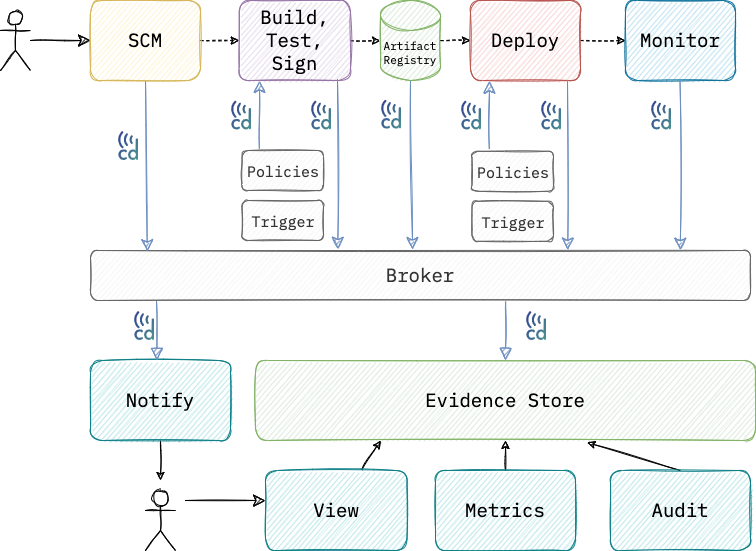
\includegraphics[width=0.80\paperwidth]{img/cdevents-4-interoperability.png}
  \end{textblock*}
\end{grayframe}
\note[itemize]{
  \item Observability of CI/CD pipelines
  \begin{itemize}
    \item Metrics
    \item Notification
    \item Single View
  \end{itemize}
  \item Metrics: unique combinations of tools
  \item Notifications: template to fetch data from multiple sources
  \item Build a diagram, show the need for interoperability
}

\begin{lpicrblack}[whycdevents]{}%
  {%
  \begin{itemize}
    \item Event driven workflows
    \begin{itemize}
      \item Scalable, Decoupled
      \item Flexible
      \item Policy Driven
    \end{itemize}
    \item Observability
    \begin{itemize}
      \item Metrics
      \item Notifications
      \item Single View
    \end{itemize}
    ~ \\
    \textbf{Interoperability!} \\
  \end{itemize}
  }%
  {0.60}
  \frametitle{~~~~~~~~~~~~~~~~~~~~~~~~~~~~~~~~~~~~~~~~~~~~~~~~~~~~~~~~~~~~~~~~~~~~~~~~~Why CDEvents}
\end{lpicrblack}
\note[itemize]{
  Event driven workflows
  \begin{itemize}
    \item Scalable
    \item Decoupled
    \item Flexible
    \item Policy Driven
  \end{itemize}
  Observability of CI/CD pipelines
  \begin{itemize}
    \item Metrics
    \item Notification
    \item Single View
  \end{itemize}
}

\begin{lgrayframerpic}[jon-tyson-FlHdnPO6dlw-unsplash]{%
  Photo by \href{https://unsplash.com/@jontyson}{\underline{Jon Tyson}}, CC0
  }%
  {%
  \begin{itemize}
    \item Interoperability and Events Special Interest Groups
    \item First Commit Oct 2020 
    \item Incubated at the CDF since 2022
  \end{itemize}
  ~\\
  \begin{itemize}
    \item Release v0.1 announced at the CDSummit in Detroit
    \begin{itemize}
      \item Orchestration
      \item Software Configuration Management
      \item Continuous Integration \& Deployment
      \item CloudEvents Binding
      \item Golang SDK
      \item DevOps Metrics
    \end{itemize}
  \end{itemize}
  }%
  {0.65}
  \frametitle{History of CDEvents}
\end{lgrayframerpic}
\note[itemize]{
  \item Incubated at the CDF since 2022
  \item CDEventsCon May 2022
  \item Release v0.1, CDSummit in Detroit, Nov 2022
  \item Scope:
  \begin{itemize}
    \item Orchestration
    \item Software Configuration Management
    \item Continuous Integration
    \item Continuous Deployment
  \end{itemize}
  DevOps Metrics:
  \begin{itemize}
    \item Lead Time for Changes
    \item Deployment Frequency
  \end{itemize}
}

\section{What's New}
\begin{sectionwithpiclargecentral}[josh-sorenson-MjIMc6uhwrE-unsplash.jpg]{Photo by \href{https://unsplash.com/@joshsorenson}{\underline{Josh Sorenson}}, CC0}
\end{sectionwithpiclargecentral}

\begin{tpicstripedframe}%
  {cdevents-banner.png}
  {%
  Incident Events:
  \begin{itemize}
    \item Continuous Operations
    \item Modeled after DORA
    \item Remediation Automation
  \end{itemize}
  }%
  {%
  Test Events:
  \begin{itemize}
    \item Notifications
    \item Test Driven Automation
    \item Metrics
  \end{itemize}
  }%
  {%
  Software Supply Chain Security \\
  \vspace{0.01\textheight}
  \begin{itemize}
    \item Artifact Signed event
    \item Build \& Deployment Automation
  \end{itemize}
  }%
  {%
  Quality of life improvements
  \begin{itemize}
    \item Improved readability
    \item Examples for each event
    \item Refreshed web site
  \end{itemize}
  }%
\end{tpicstripedframe}
\note[itemize]{
  \item Improved readability of the specification
  \item Examples for each event type
  \item Refreshed web site
  \item Golang SDK v0.3, now generated from JSON schemas
  \item Java SDK published to Maven Central
  \item Python SDK published to PyPi
}

\begin{blackframe}
  \frametitle{SDKs}
\end{blackframe}
\note[itemize]{
  \item Golang SDK v0.3, now generated from JSON schemas
  \item Java SDK published to Maven Central
  \item Python SDK published to PyPi
  \item CDEventer?
}

\section{Tools Adoption}
\begin{sectionwithpiclargecentral}[clay-banks-LjqARJaJotc-unsplash.jpg]{Photo by \href{https://unsplash.com/@claybanks}{\underline{Clay Banks}}, CC0}
\end{sectionwithpiclargecentral}

\begin{blackframe}
  \frametitle{Overview}
\end{blackframe}
\note[itemize]{
  \item Jenkins
  \item Spinnaker
  \item Testkube
  \item Tekton (experimental)
  \item Argo Rollout (PoC)
  \item Flux (PoC)
}

\begin{blackframe}
  \frametitle{Jenkins}
\end{blackframe}
\note[itemize]{
  \item Check with Jamie for diagram
}

\begin{blackframe}
  \frametitle{Spinnaker}
\end{blackframe}
\note[itemize]{
  \item Check with Ben, can we mention Apple
}

\begin{blackframe}
  \frametitle{Testkube}
\end{blackframe}
\note[itemize]{
  \item Check with Bruno for diagram
}

\begin{blackframe}
  \frametitle{Tekton}
\end{blackframe}
\note[itemize]{
  \item CI Notifications
  \item CD Notifications
  \item Release automation
}

\begin{blackframe}
  \frametitle{Lessons Learnt}
\end{blackframe}
\note[itemize]{
  \item How to adopt CDEvents
  \item Start small, iterate
  \item Get adopters involved
  \item Collaboration between open source communmities
  \item Spec Examples
  \item SDK docs and Examples
  \item SDK conformance
  \item Generate docs and SDKs from single source
}

% \begin{lpicrblack}[benjamin-rascoe-braMiRFMHPk-unsplash]{Photo by \href{https://unsplash.com/@dapperprofessional}{\underline{Benjamin Rascoe}}, CC0}%
%   {%
%   Website refresh
%   \begin{itemize}
%     \item Target Audiences
%     \item Simplified DevEx
%     \item Accessibility 
%   \end{itemize}
%   ~ \\
%   SDKs
%   \begin{itemize}
%     \item Java SDK for v0.1 (Spinnaker, Fidelity)
%   \end{itemize}
%   ~ \\
%   Specification
%   \begin{itemize}
%     \item Incidents \& Remediations
%     \item Connecting events
%   \end{itemize}
%   ~ \\
%   Tools
%   \begin{itemize}
%     \item Spinnaker
%   \end{itemize}
%   }%
%   {0.3}
%   \frametitle{~~~~~~~~~~~~~~~~~~~~~~~~~~~~~~~~~~~~~~~~~~~~~~~~~~~~~~~~~~Working In Progress}
% \end{lpicrblack}

\section{Roadmap}
\begin{sectionwithpiclargecentral}[dimitar-donovski-yrjB4dYWUZU-unsplash.jpg]{Photo by \href{https://unsplash.com/@dmtrdon}{\underline{Dimitar Donovski}}, CC0}
\end{sectionwithpiclargecentral}

\begin{stripedframe}%
  {%
  CDEvents Roadmap \\
  v0.4 and beyond \\
  ~
  }%
  {%
  Supply Chain Security
  \begin{itemize}
    \item SBOM, Provenance, Signatures
  \end{itemize}
  \begin{itemize}
    \item Signed Events
  \end{itemize}
  }%
  {%
  E2E Supply Chain \\
  ~
  \begin{itemize}
    \item Requirements
    \item Releases
    \item Production
    \item Incidents
    \item Remediations
  \end{itemize}
  }%
  {%
  New features \\
  ~
  \begin{itemize}
    \item Compositions
    \item Links, Workflow IDs
    \item SDKs
    \item Policy Driven Workflow
  \end{itemize}
  }%
  {%
  Data Model \\
  ~
  \begin{itemize}
    \item SCM Events
    \item Tests
  \end{itemize}
  Documentation:
  \begin{itemize}
    \item Architecture
    \item Examples
  \end{itemize}
  }%
\end{stripedframe}
\note[itemize]{
  \item Roadmap to be updated
  \item SDK Rust/JS?
}

\begin{blackframe}
  \frametitle{Collaborations}
\end{blackframe}
\note[itemize]{
  \item CDF, Reference Architecture
  \item Workshop working group
  \item VSMI
  \item CNCF TAG App Delivery
}

\begin{stripedframe}%
  {%
  Community
  ~ \\
  ~ \\
  }%
  {%
  CDF \\
  ~
  \begin{itemize}
    \item SIG Interop
    \item SIG Supply Chain
    \item SIG Best Practices
  \end{itemize}
  }%
  {%
  Tools communities \\
  ~
  \begin{itemize}
    \item Tekton
    \item Spinnaker
    \item Shipwright
    \item Jenkins
    \item Jenkins X
    \item Flux, Argo
  \end{itemize}
  }%
  {%
  Companies \\
  ~
  \begin{itemize}
    \item Ericsson
    \item IBM / RedHat
    \item doWhile
    \item Apple
    \item VMWare
    \item Fidelity
    \item SAS
  \end{itemize}
  }%
  {%
  Get Involved!! \\
  ~
  \begin{itemize}
    \item Specification
    \item SDKs (Rust, JS, Ruby, C\#)
    \item Tools
    \item Proof-of-concepts
    \item End users
  \end{itemize}
  }%
\end{stripedframe}
\note[itemize]{
  \item To be updated, maybe change to an how to contribute
}

\section[Thank You]{Thank You!}

\begin{sectionwithpiclargecentral}[carl-jorgensen-5nrnxx_tWe8-unsplash.jpg]{Brecon Beacons, Walse, Photo by \href{https://unsplash.com/@scamartist}{\underline{Carl Jorgensen}}, CC0}
\end{sectionwithpiclargecentral}

\begin{blackframe}
  \frametitle{References}
  \begin{itemize}
    \item \href{https://cdevents.dev}{cdevents.dev}
    \item \href{https://github.com/cdevents/spec/blob/main/CDEvents_Whitepaper.pdf}{github.com/cdevents/spec/blob/main/CDEvents\_Whitepaper.pdf}
    \item \href{https://github.com/cdevents/sdk-go}{github.com/cdevents/sdk-go}
    \item \href{https://github.com/cdevents/sdk-python}{github.com/cdevents/sdk-python}
    \item \href{https://github.com/cdevents/sdk-java}{github.com/cdevents/sdk-java}
  \end{itemize}
  ~ \\
  Andrea Frittoli \\
  Developer Advocate @ IBM\\
  andrea.frittoli@uk.ibm.com \\
  \faTwitter ~@blackchip76 | \faGithub ~afrittoli | \faLinkedin ~andreafrittoli
\end{blackframe}

\end{document}
